\section{Automap: Using Autoencoders to Learn an Evolvable Genotype-Phenotype Map}

\begin{frame}{Remember This?}

\begin{figure}
\begin{subfigure}[b]{\textwidth}
\foreach \n in {6,...,1}{%
\includegraphics[width=0.167\textwidth]{straight-guy/latent-\n}%
}%
\caption{latent-space interpolation}
\end{subfigure}

\uncover<2>{
\begin{subfigure}[b]{\textwidth}
\foreach \n in {1,...,6}{%
\includegraphics[width=0.167\textwidth]{straight-guy/linear-\n}%
}%
\caption{pixel-space interpolation}
\end{subfigure}
}

\caption{
Comparison of latent- and pixel-space interpolations.
Graphics adapted from \cite{white2016sampling}.
}
\end{figure}

\end{frame}

\begin{frame}{Bottlenecked G-P Map: Implementation}

\begin{figure}
  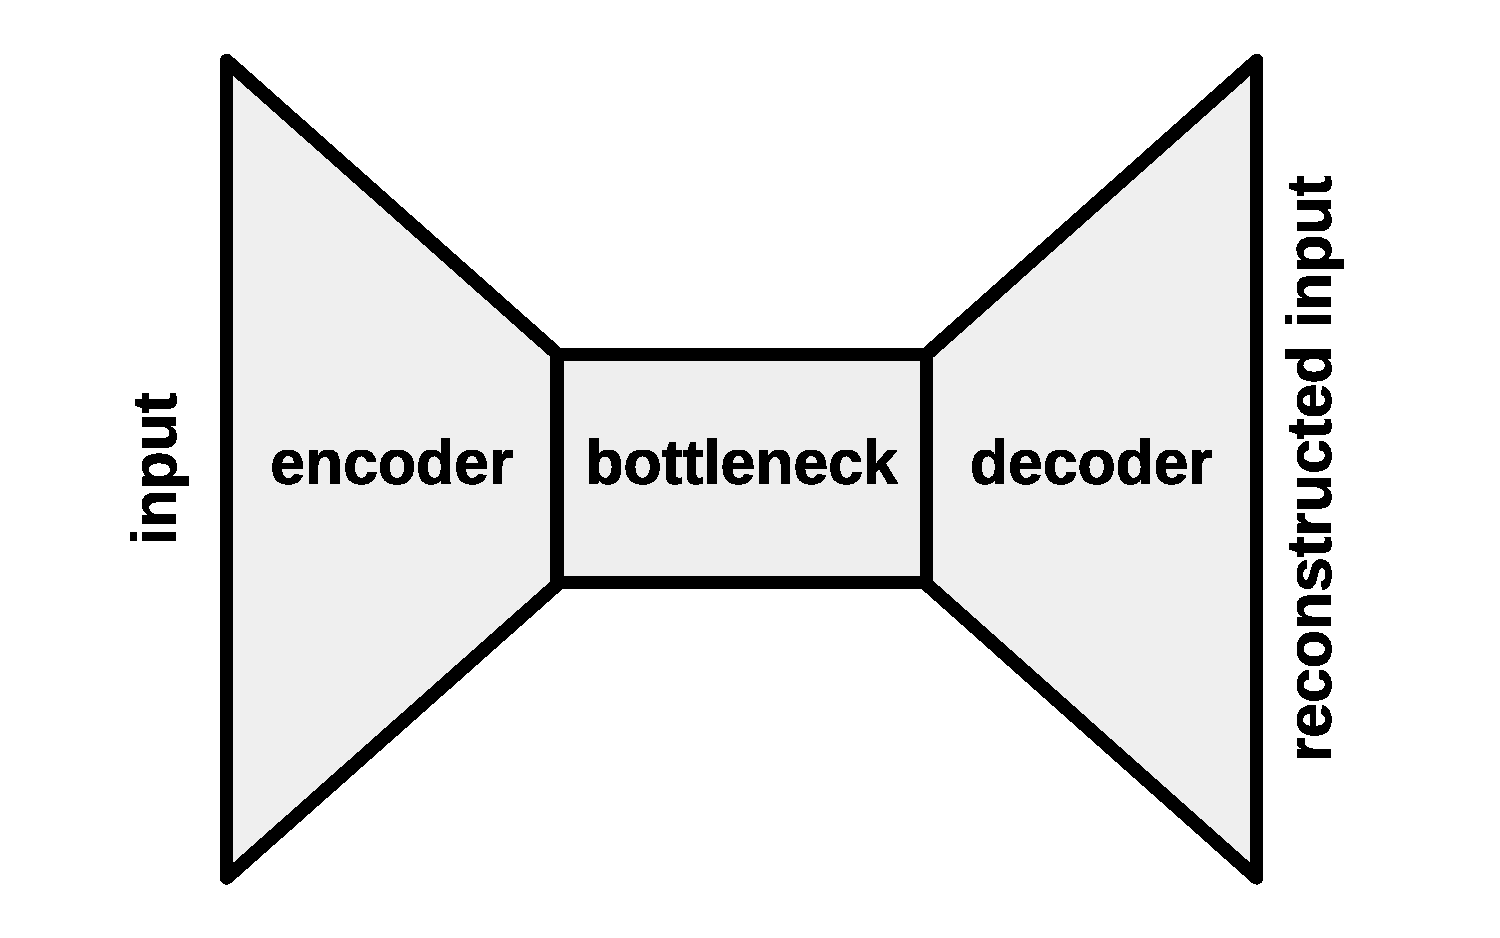
\includegraphics[width=\linewidth]{img/bottleneck}
  \caption{
    Schematic of a bottlenecked autoencoder.
  }\label{fig:bottleneck}
\end{figure}


\end{frame}

\begin{frame}{Bottlenecked G-P Map: Implementation}

\begin{figure}
  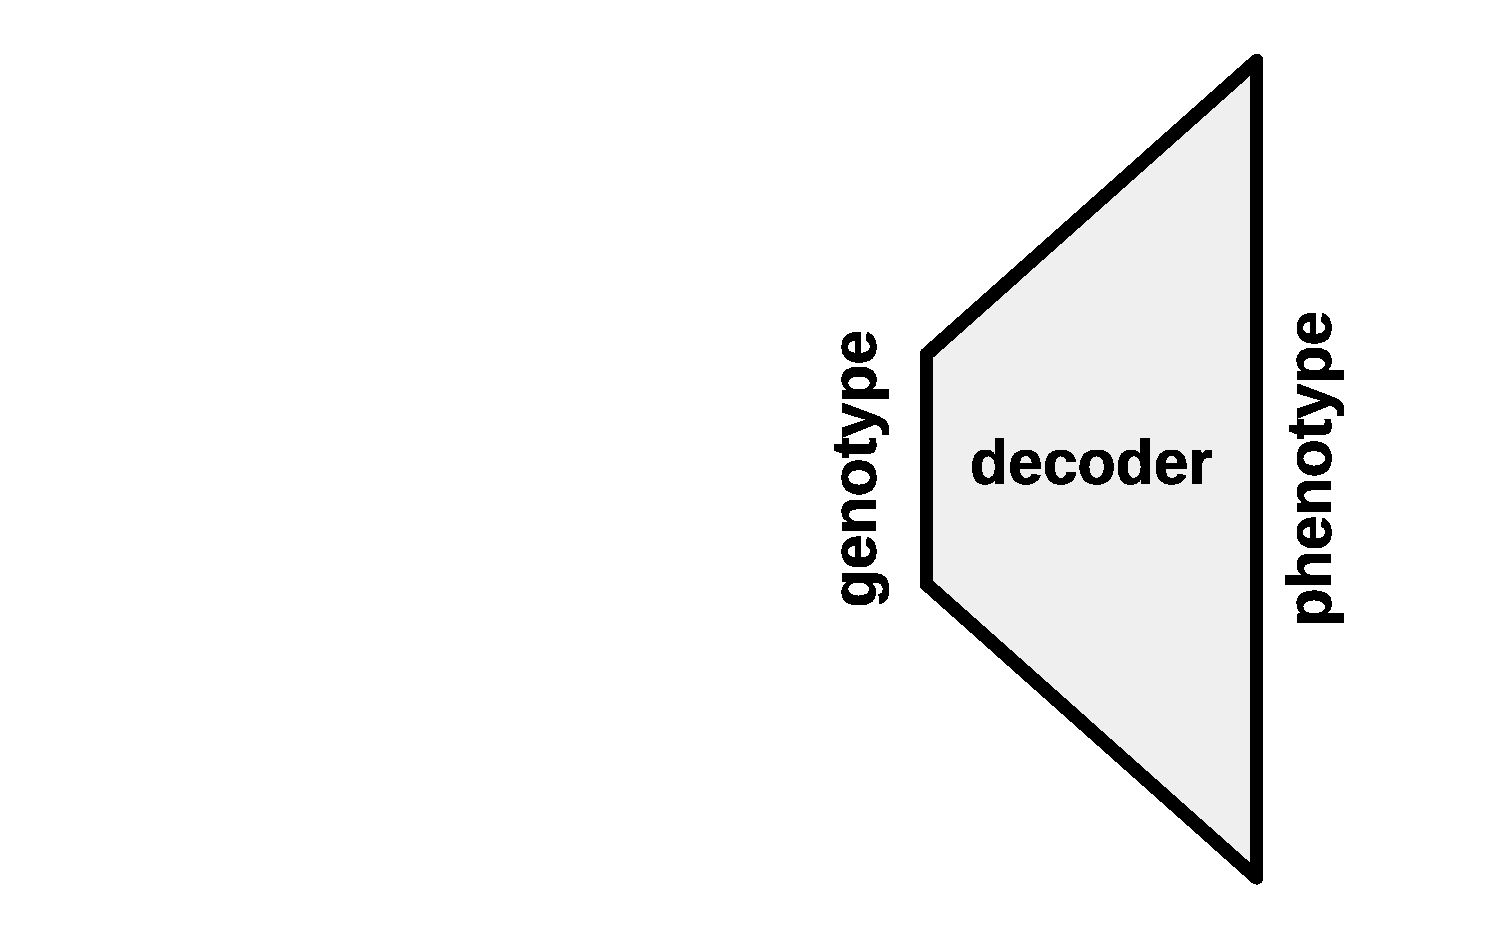
\includegraphics[width=\linewidth]{img/bottleneck_map}
  \caption{
    Schematic of a genotype-phenotype map constructed with a bottlenecked autoencoder.
  }\label{fig:bottleneck_map}
\end{figure}


\end{frame}

\begin{frame}{Bottlenecked G-P Map: Evolvability}
\begin{figure}
\begin{columns}
\begin{column}{0.7\textwidth}
  \includegraphics[width=\textwidth]{landscape-bottleneck/landscape-1}%
\end{column}
\begin{column}{0.3\textwidth}
\caption{
A hypothetical fitness landscape.
}
\end{column}
\end{columns}
\end{figure}
\end{frame}

\begin{frame}{Bottlenecked G-P Map: Evolvability}
\begin{figure}
\begin{columns}
\begin{column}{0.7\textwidth}
  \includegraphics[width=\textwidth]{landscape-bottleneck/landscape-2}%
\end{column}
\begin{column}{0.3\textwidth}
\caption{
Hypothetical evolutionary end-state of a single population on a fitness landscape.
}
\end{column}
\end{columns}
\end{figure}
\end{frame}

\begin{frame}{Bottlenecked G-P Map: Evolvability}
\begin{figure}
\begin{columns}
\begin{column}{0.7\textwidth}
  \includegraphics[width=\textwidth]{landscape-bottleneck/landscape-3}%
\end{column}
\begin{column}{0.3\textwidth}
\caption{
Hypothetical evolutionary end-state of several populations on a fitness landscape.
}
\end{column}
\end{columns}
\end{figure}
\end{frame}

\begin{frame}{Bottlenecked G-P Map: Evolvability}
\begin{figure}
  \includegraphics<1>[width=\textwidth,trim={0 4cm 0 4cm },clip]{landscape-bottleneck/landscape-4}%
  \includegraphics<2>[width=\textwidth,trim={0 4cm 0 4cm },clip]{landscape-bottleneck/landscape-5}%
  \includegraphics<3>[width=\textwidth,trim={0 4cm 0 4cm },clip]{landscape-bottleneck/landscape-6}%
  \includegraphics<4>[width=\textwidth,trim={0 4cm 0 4cm },clip]{landscape-bottleneck/landscape-7}%
  \includegraphics<5>[width=\textwidth,trim={0 4cm 0 4cm },clip]{landscape-bottleneck/landscape-8}%
\caption{
Hypothetical mutational trajectory on a fitness landscape with denoising genotype-phenotype map.
}
\end{figure}
\end{frame}

\begin{frame}{Remember This?}
  \vspace{2ex}
  \begin{figure}
  \begin{columns}
  \begin{column}{0.3\textwidth}
  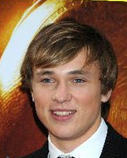
\includegraphics[width=\textwidth]{reconstruct/original-boy}
  \end{column}
  \begin{column}{0.05\textwidth}
  \centering
  \rotatebox{90}{Corrupt}\\
  
\includegraphics[width=\textwidth]{arrow}
  \end{column}
  \begin{column}{0.3\textwidth}
  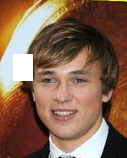
\includegraphics[width=\textwidth]{reconstruct/corrupted-boy}
  \end{column}
  \begin{column}{0.05\textwidth}
  \centering
  \rotatebox{90}{Autoencoder}\\
  
\includegraphics[width=\textwidth]{arrow}
  \end{column}
  \begin{column}{0.3\textwidth}
  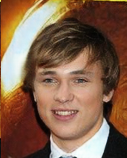
\includegraphics[width=\textwidth]{reconstruct/reconstructed-boy}
  \end{column}
  \end{columns}
  \vspace{1ex}
  \caption{
  Autoencoder restoring masked section of image.
  Graphics from \cite{white2016sampling}.
  }
  \end{figure}

\end{frame}

\begin{frame}{Denoising G-P Map: Implementation}

\begin{figure}
  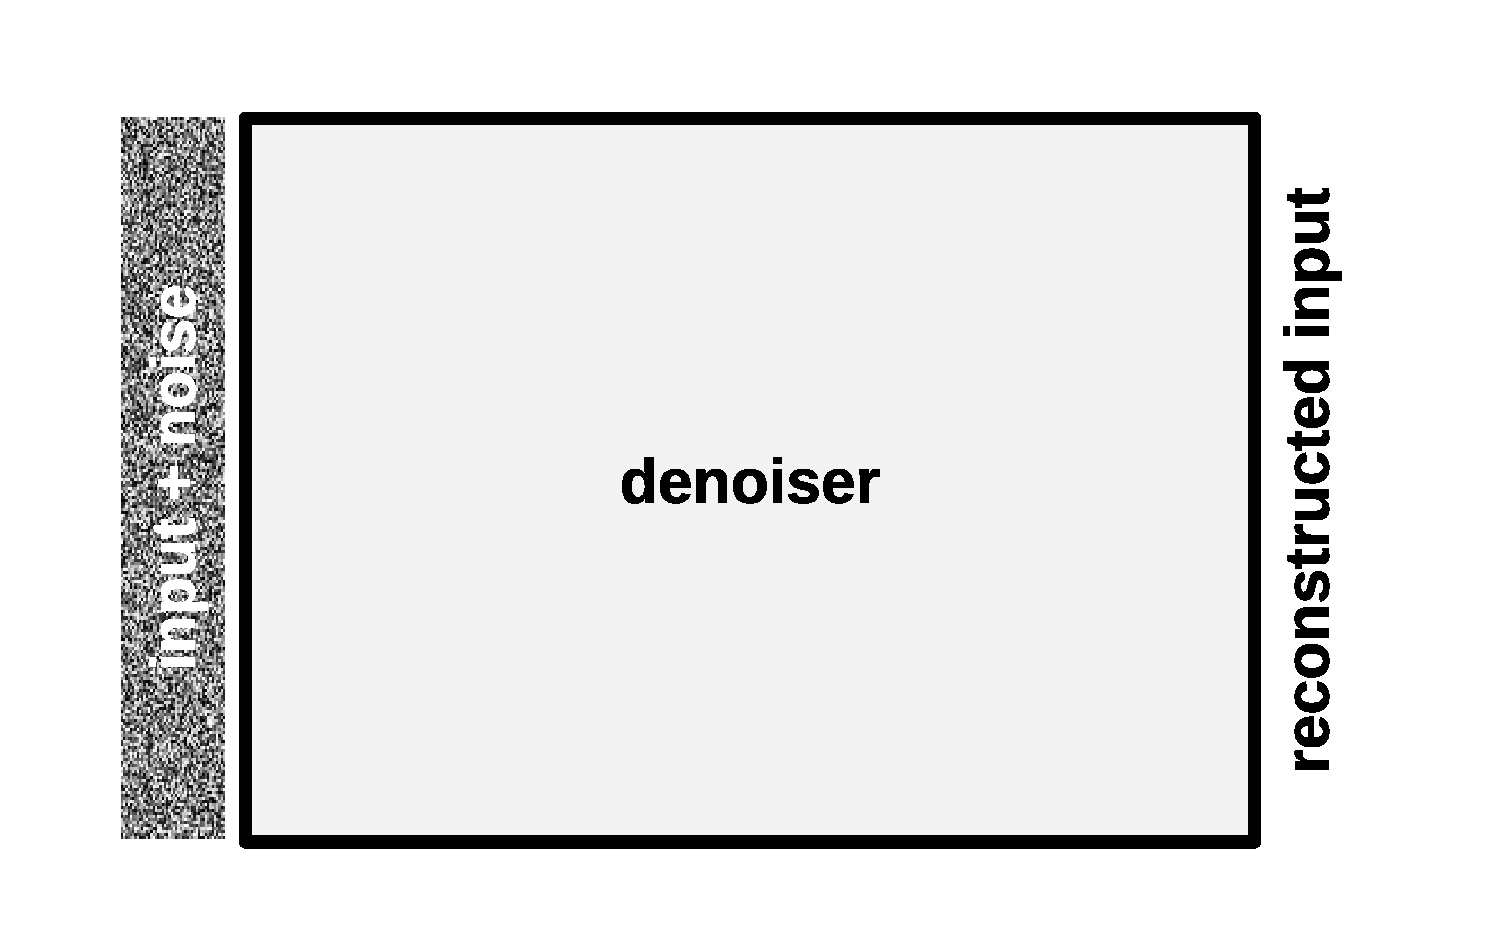
\includegraphics[width=\linewidth]{img/denoiser}
  \caption{
    Schematic of a denoising autoencoder.
  }\label{fig:denoiser}
\end{figure}


\end{frame}

\begin{frame}{Denoising G-P Map: Implementation}

\begin{figure}
  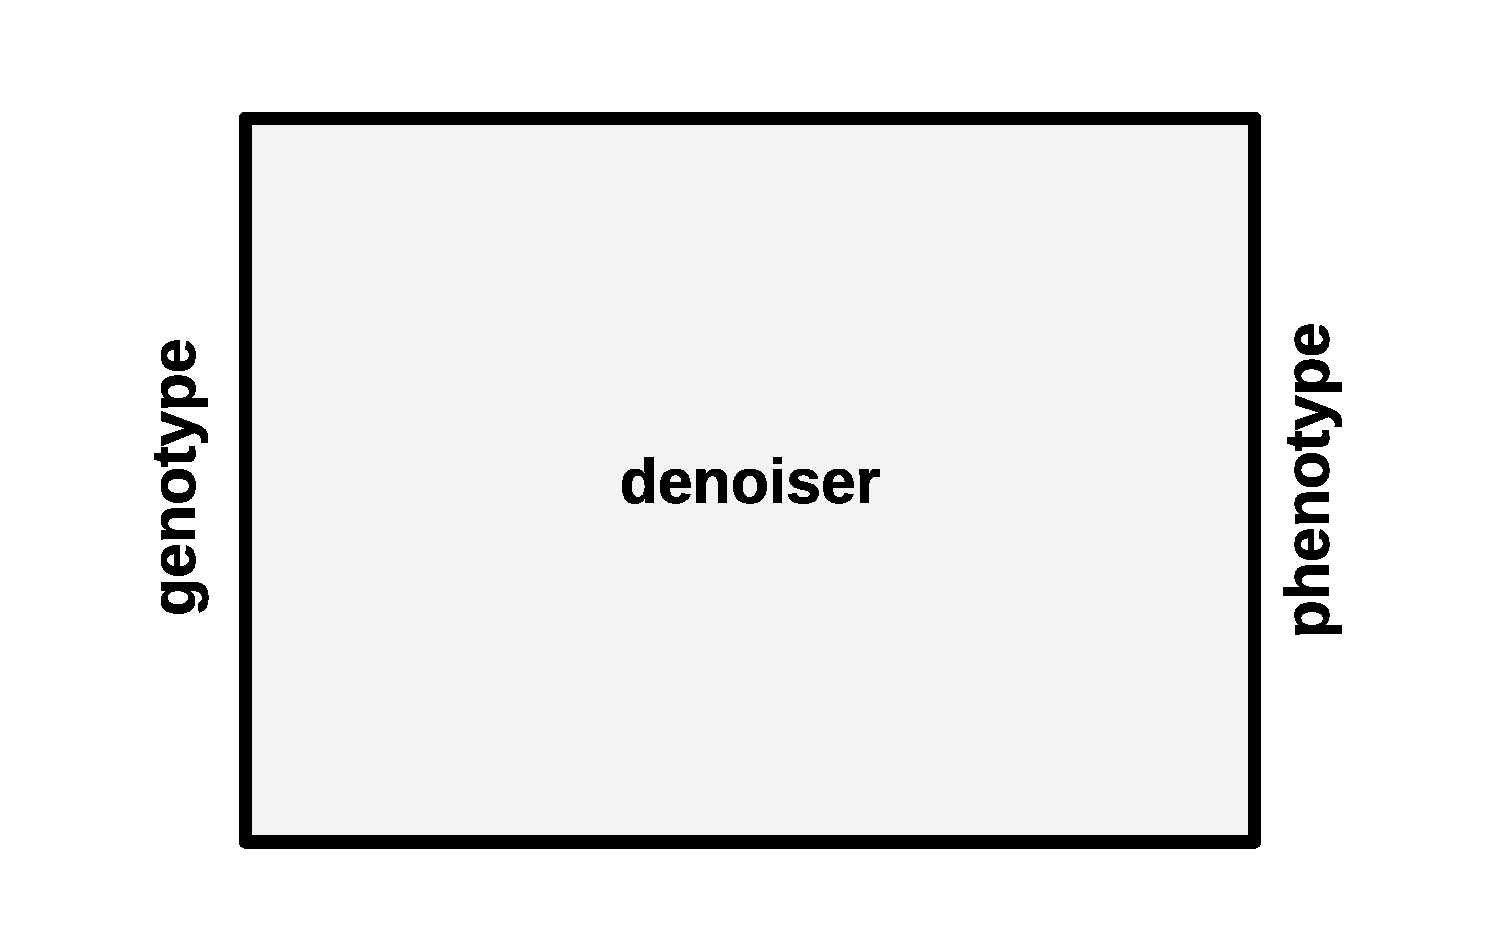
\includegraphics[width=\linewidth]{img/denoiser_map}
  \caption{
    Schematic of a genotype-phenotype map constructed with a denoising autoencoder.
  }\label{fig:denoiser_map}
\end{figure}


\end{frame}

\begin{frame}{Denoising G-P Map: Evolvability}

\begin{figure}

\begin{columns}
\begin{column}{0.6\textwidth}
  \includegraphics[width=\textwidth]{landscape-denoise/landscape-1}%
\end{column}
\begin{column}{0.4\textwidth}
\caption{
A hypothetical fitness landscape.
}
\end{column}
\end{columns}

\end{figure}

\end{frame}
\begin{frame}{Denoising G-P Map: Evolvability}

\begin{figure}

\begin{columns}
\begin{column}{0.6\textwidth}
  \includegraphics[width=\textwidth]{landscape-denoise/landscape-2}%
\end{column}
\begin{column}{0.4\textwidth}
\caption{
Hypothetical evolutionary end-state of a single population on a fitness landscape.
}
\end{column}
\end{columns}

\end{figure}

\end{frame}
\begin{frame}{Denoising G-P Map: Evolvability}

\begin{figure}

\begin{columns}
\begin{column}{0.6\textwidth}
  \includegraphics[width=\textwidth]{landscape-denoise/landscape-3}%
\end{column}
\begin{column}{0.4\textwidth}
\caption{
Hypothetical evolutionary end-state of several populations on a fitness landscape.
}
\end{column}
\end{columns}

\end{figure}

\end{frame}
\begin{frame}{Denoising G-P Map: Evolvability}

\begin{figure}
  \begin{columns}
  \begin{column}{0.6\textwidth}
  \includegraphics<1>[width=\textwidth]{landscape-denoise/landscape-4}%
  \includegraphics<2>[width=\textwidth]{landscape-denoise/landscape-5}%
  \includegraphics<3>[width=\textwidth]{landscape-denoise/landscape-6}%
  \includegraphics<4>[width=\textwidth]{landscape-denoise/landscape-7}%
  \includegraphics<5>[width=\textwidth]{landscape-denoise/landscape-8}%
\end{column}
\begin{column}{0.4\textwidth}
\caption{
Hypothetical mutational trajectory on a fitness landscape with denoising genotype-phenotype map.
}
\end{column}
\end{columns}

\end{figure}

\end{frame}

\begin{frame}{Autoencoder G-P Maps: Training}
\Large

We need examples of good solutions to train autoencoder.

\pause

How to get training data?

\pause

\begin{itemize}[<+->]
\item survey local fitness peaks
\begin{itemize}
  \item repeated evolutionary runs with direct encoding
  \item repeated evolutionary runs with manually-designed indirect encoding
\end{itemize}
\item harness pre-existing data
\begin{itemize}
  \item ex. face images
\end{itemize}
\end{itemize}

\end{frame}
